\documentclass{article}

\usepackage[preprint]{nips_2018}
% to avoid loading the natbib package, add option nonatbib:
% \usepackage[nonatbib]{nips_2018}

\usepackage[utf8]{inputenc} % allow utf-8 input
% \usepackage[T1]{fontenc}    % use 8-bit T1 fonts
\usepackage{hyperref}       % hyperlinks
\usepackage{url}            % simple URL typesetting
\usepackage{booktabs}       % professional-quality tables
\usepackage{amsfonts}       % blackboard math symbols
\usepackage{nicefrac}       % compact symbols for 1/2, etc.
\usepackage{microtype}      % microtypography
\usepackage{amsmath}
\usepackage{mathtools}
\usepackage{float}
\usepackage{graphicx}
\usepackage{algorithm}
\usepackage{algpseudocode}
\usepackage{cleveref}       % this package must be loaded at the last
\usepackage{subcaption}
\usepackage{enumitem}
\usepackage{verbatim}
\usepackage{algorithmicx}
\usepackage{listings}       % for adding source code
\usepackage{courier}
\usepackage{xcolor}

\definecolor{codegreen}{rgb}{0,0.6,0}
\definecolor{codegray}{rgb}{0.5,0.5,0.5}
\definecolor{codepurple}{rgb}{0.58,0,0.82}

\lstset
{ %Formatting for code in appendix
    language=Python,  
    commentstyle=\color{codegreen},
    keywordstyle=\color{magenta},
    numberstyle=\tiny\color{codegray},
    stringstyle=\color{codepurple},
    basicstyle=\footnotesize\ttfamily,
    numbers=left,
    stepnumber=1,
    showstringspaces=false,
    tabsize=1,
    breaklines=true,
    breakatwhitespace=false,
}


\DeclareMathOperator*{\argmax}{argmax}
\newlist{steps}{enumerate}{1}
\setlist[steps, 1]{label = Step \arabic*:}

\title{EL2805 Lab2 Report}

\author{
  Chun Hung Lin \\
  \texttt{chlin3@kth.se} \\
  \texttt{199109301458}
  \And
  Yini Yang \\
  \texttt{yiniy@kth.se} \\
  \texttt{199504244188}
}

\begin{document}
\maketitle

\section{Problem 1}

\subsection{Formulate the problem as a RL problem}

This problem can be formulated as an episodic RL problem.

\textbf{State space:}

Here we use the observations from openAI as states. The state space $S$ can be described as follows:
$$ S = \{S_i=(p,v,\theta,v_{tip})|p\in[-4.8,4.8],v\in[-\infty,\infty],\theta\in[-24,24],v_{tip}\in[-\infty,\infty],i=0,1,\cdots\}$$
where $p,v$ refer to the position and velocity of the cart respectively, while $\theta,v_{tip}$ correspond to the angle and velocity at tip of the pole.

\textbf{Action space:}
$$A=\{0,1\}$$
where $0$ means to push cart to the left and $1$ means to push cart to the right.

\textbf{Reward:}

The reward can be formulated as a function of $r: S\times A\rightarrow \mathbb{R}$.
\begin{equation*}
  r(s, :) =
  \begin{cases}
    1  \quad &-2.4\leq p\leq 2.4, -12.5\leq \theta \leq 12.5\\
    0    \quad &\textup{otherwise}
  \end{cases}
\end{equation*}

\textbf{Termination:}

The episode terminates after 200 steps or once the agent receives 0 reward for the first time.

\textbf{Problem analysis:}

We cannot use the standard reinforcement learning method to solve this problem.
It is because the state variables are continuous instead of discrete.
Therefore the Q-learning and SARSA for constructing a tabular state-action value function (i.e. Q-function)
are not suitable for this case.

Using a neural network to approximate the Q-function is robust and more powerful. 
As the universal approximation theorem states that any continuous functions on the subset $\mathbb R^n$ 
can be approximated by a finite number of neurons and certain activation functions.

\subsection{Pseudo-code for DQN}
The pseudo-code is mentioned in algorithm \ref{algo:DQN}

\begin{algorithm}[!htbp]
  \caption{DQN}
  \label{algo:DQN}
  \begin{algorithmic}[1]
    \State Initialize $\phi,\phi'$   \Comment{agent.build\_model() and DQNAgent constructor}
    \For{each episode $k=1,2,\cdots$}
      \For{$t=0, \cdots, N$}
        \State Get the $\epsilon$-greedy action $a_t=\pi(s_t)$ according to $Q_{\phi}(s_t,a_t)$ \Comment{Line 281}
        \State Obtain observations $(s_t,a_t,r_t,s_{t+1})$    \Comment{Line 282-283}
        \State Add $(s_t,a_t,r_t,s_{t+1})$ to the memeory set \Comment{Line 287}
        \For{$i=1,\cdots,|B|$}  \Comment{In agent.train\_model}
          \State Sample $(s_t,a_t,r_t,s_{t+1})$ from memory
          \Comment{Line 127}
          \State Calculate $Q_{\phi}(s_t,a_t)$ and $Q_{\phi'}(s_{t+1},a_t)$ according to the network
          \Comment{Line 159,161}
          \State Calculate the target value:
            \Comment{Line 168-175} 
            \begin{equation*}
              y_t =
              \begin{cases}
                r_t       \quad  &\textup{if episode stops in $s_{t+1}$} \\
                r_t + \lambda\max_{b}Q_{\phi'}(s_{t+1}, a_t)    \quad &\textup{otherwise}
              \end{cases}
            \end{equation*}
          \State Update $\phi$:
          $$\phi\leftarrow\phi-\alpha(Q_{\phi}(s_t,a_t)-y_i)\nabla_{\phi}Q_{\phi}(s_t,a_t)$$ \Comment{Line: 178, self.model.fit(...)}
        \EndFor
      \EndFor
      \State Update $\phi'$ every $C$ steps: $\phi'\leftarrow\phi$ \Comment{Line: 283-284}
      \If {\textit{terminated conditions satisfied}}
        \State \textbf{break}
      \EndIf
    \EndFor
  \end{algorithmic}
\end{algorithm}

\subsection{Impact of the number of nodes and hidden layers}

Five different FNN structures have been tested in this section. The average Q values and scores in the
training process have been visualized from Figure \ref{1 layer FNN} to Figure \ref{multi layers FNN}.

\begin{figure}[!htbp]
  \centering
  \begin{subfigure}{\textwidth}
    \begin{minipage}{0.5\textwidth}
      \centering
      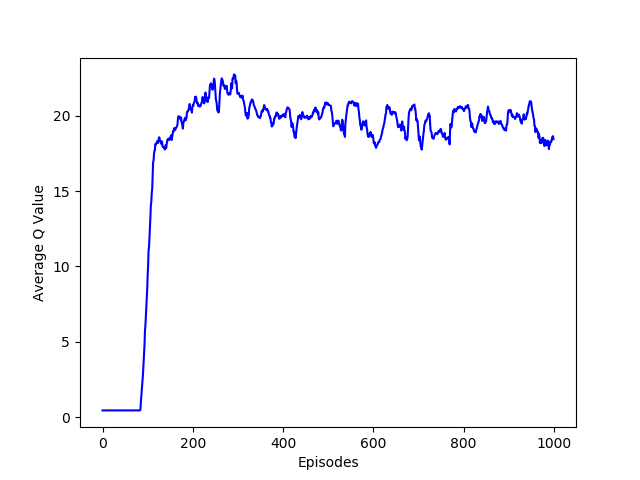
\includegraphics[scale=0.45]{../experiments/nn_size_16/qvalues.png}
    \end{minipage}
    \begin{minipage}{0.5\textwidth}
      \centering
      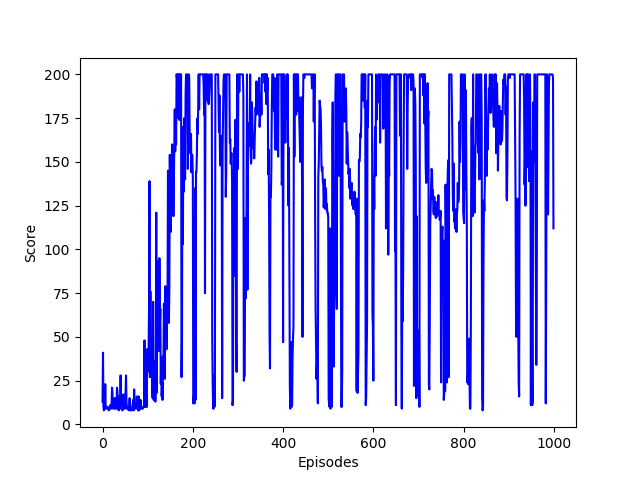
\includegraphics[scale=0.45]{../experiments/nn_size_16/scores.png}
    \end{minipage}
    \caption{One hidden layer with 16 nodes.}
  \end{subfigure}%

  \begin{subfigure}{\textwidth}
    \begin{minipage}{0.5\textwidth}
      \centering
      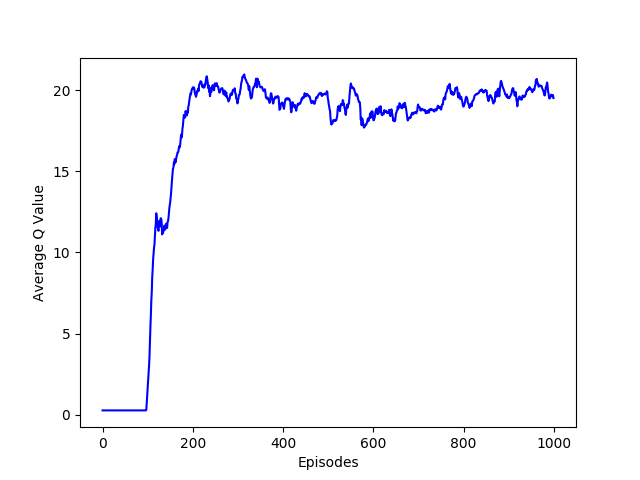
\includegraphics[scale=0.45]{../experiments/nn_size_32/qvalues.png}
    \end{minipage}
    \begin{minipage}{0.5\textwidth}
      \centering
      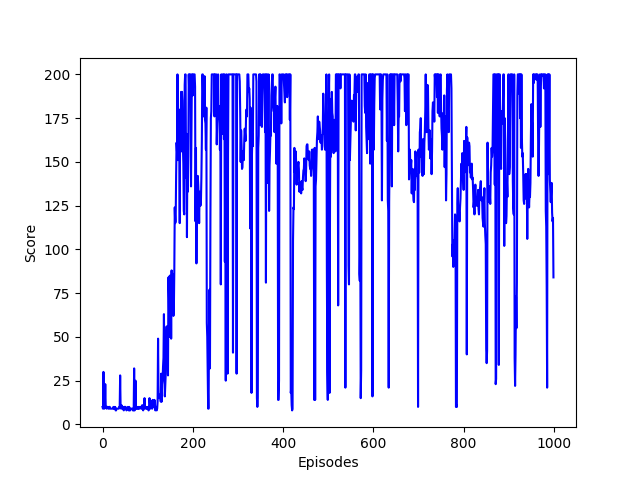
\includegraphics[scale=0.45]{../experiments/nn_size_32/scores.png}
    \end{minipage}
    \caption{One hidden layer with 32 nodes.}
  \end{subfigure}%
  \caption{Performance of FNN with one hidden layer.}
  \label{1 layer FNN}
\end{figure}

\begin{figure}[!htbp]
  \centering
  \begin{subfigure}{\textwidth}
    \begin{minipage}{0.5\textwidth}
      \centering
      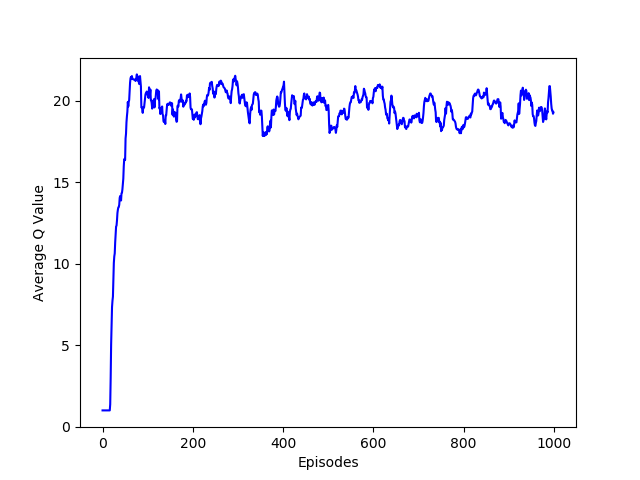
\includegraphics[scale=0.45]{../experiments/nn_size_16_16/qvalues.png}
    \end{minipage}
    \begin{minipage}{0.5\textwidth}
      \centering
      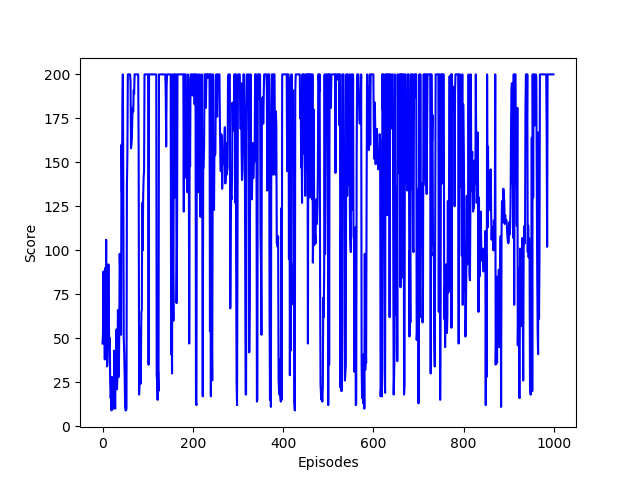
\includegraphics[scale=0.45]{../experiments/nn_size_16_16/scores.png}
    \end{minipage}
    \caption{Two hidden layers with 16-16 nodes.}
  \end{subfigure}%

  \begin{subfigure}{\textwidth}
    \begin{minipage}{0.5\textwidth}
      \centering
      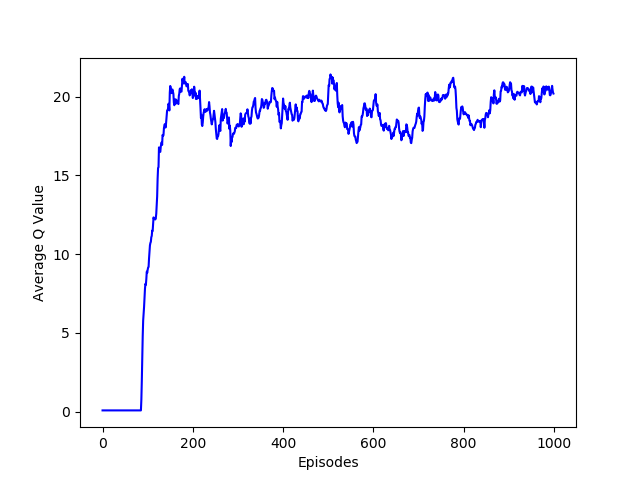
\includegraphics[scale=0.45]{../experiments/nn_size_8_16_8/qvalues.png}
    \end{minipage}
    \begin{minipage}{0.5\textwidth}
      \centering
      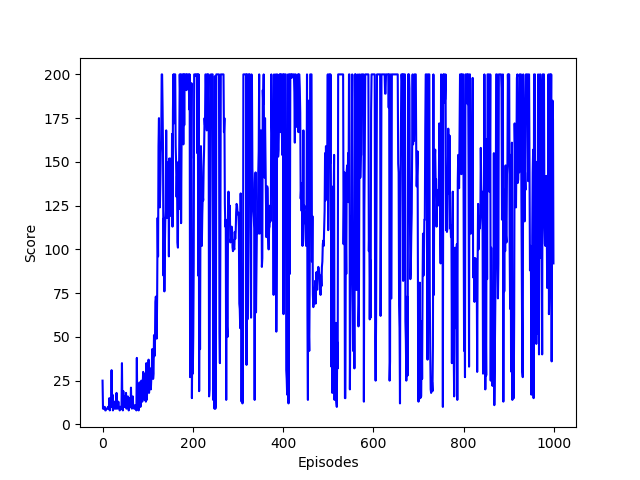
\includegraphics[scale=0.45]{../experiments/nn_size_8_16_8/scores.png}
    \end{minipage}
    \caption{Three hidden layers with 8-16-8 nodes.}
  \end{subfigure}%

  \begin{subfigure}{\textwidth}
    \begin{minipage}{0.49\textwidth}
      \centering
      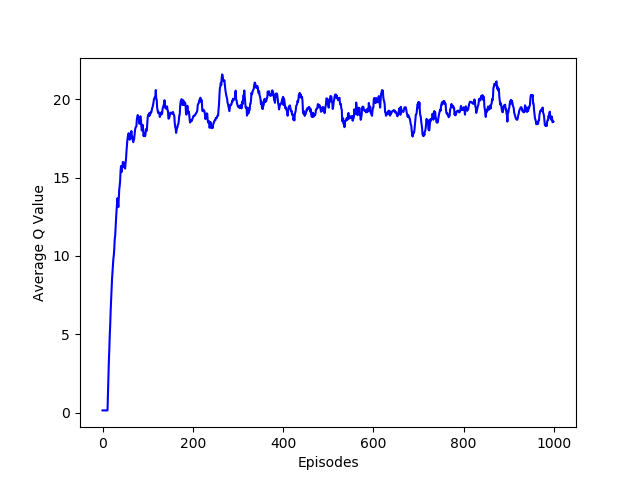
\includegraphics[scale=0.45]{../experiments/nn_size_8_16_8_4/qvalues.png}
    \end{minipage}
    \begin{minipage}{0.49\textwidth}
      \centering
      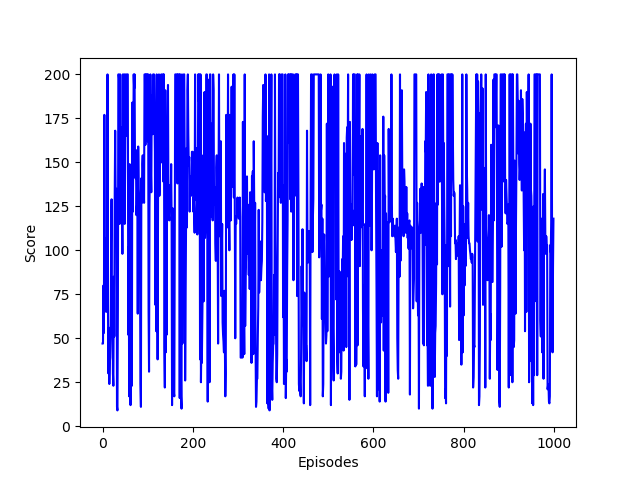
\includegraphics[scale=0.45]{../experiments/nn_size_8_16_8_4/scores.png}
    \end{minipage}
    \caption{Four hidden layers with 8-16-8-4 nodes.}
  \end{subfigure}%
  \caption{Performance of FNN with more than one hidden layer.}
  \label{multi layers FNN}
\end{figure}

When nodes and hidden layers increase, the average Q values converge faster in general. As the episodes
needed for convergence will also influenced by parameter initialization. However, from the scores grahs,
we can see the variance of scores will also rise with the complexity of the FNN structure. As a more
complicated network leads to a better fit for the model, which has less bias but higher variance.

\subsection{Impact of the discount factor, learning rate, and memory size}
\textbf{Discount factor}

Here we have tested 4 different discount factors: $0.8,0.9,0.95,0.995$. The results are show in Figure
\ref{discount factor}.

\begin{figure}[!htbp]
  \centering
  \begin{subfigure}{\textwidth}
    \begin{minipage}{0.5\textwidth}
      \centering
      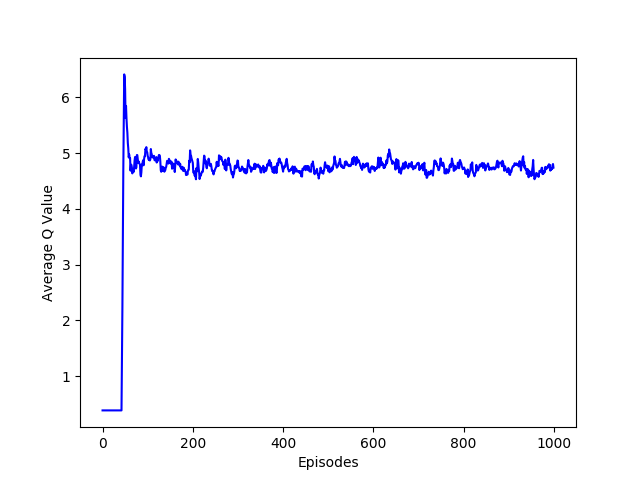
\includegraphics[scale=0.45]{../experiments/discount_factor_08/qvalues.png}
    \end{minipage}
    \begin{minipage}{0.5\textwidth}
      \centering
      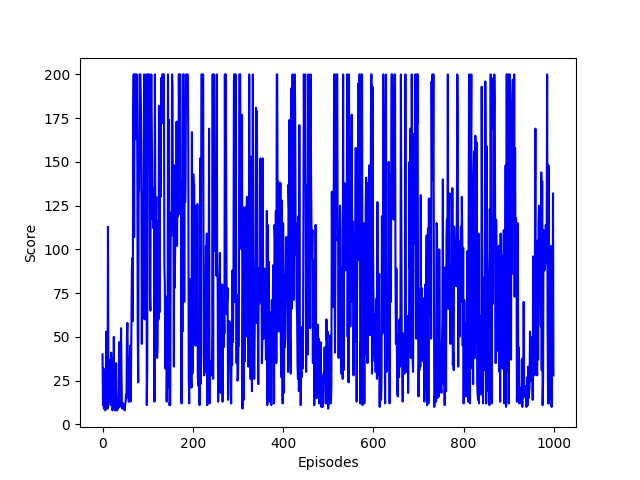
\includegraphics[scale=0.45]{../experiments/discount_factor_08/scores.png}
    \end{minipage}
    \caption{Discount factor: 0.8}
  \end{subfigure}%

  \begin{subfigure}{\textwidth}
    \begin{minipage}{0.5\textwidth}
      \centering
      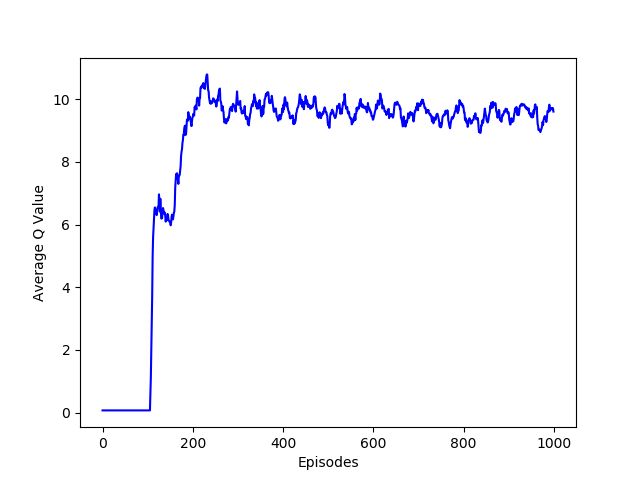
\includegraphics[scale=0.45]{../experiments/discount_factor_09/qvalues.png}
    \end{minipage}
    \begin{minipage}{0.5\textwidth}
      \centering
      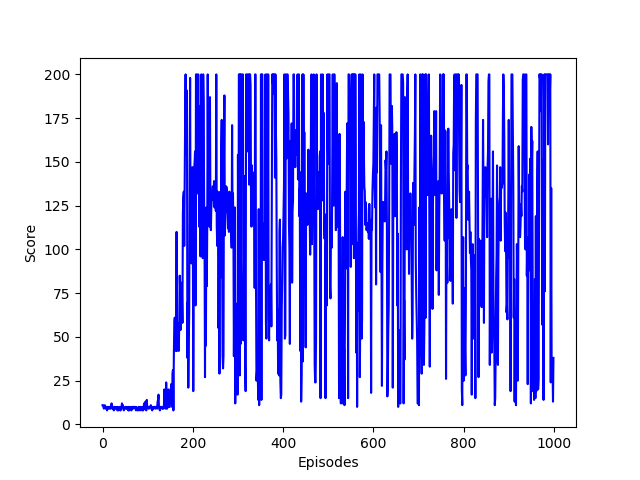
\includegraphics[scale=0.45]{../experiments/discount_factor_09/scores.png}
    \end{minipage}
    \caption{Discount factor: 0.9}
  \end{subfigure}%

  \begin{subfigure}{\textwidth}
    \begin{minipage}{0.5\textwidth}
      \centering
      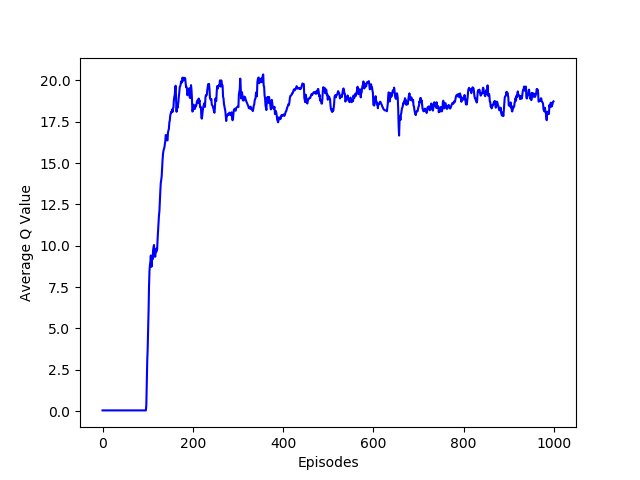
\includegraphics[scale=0.45]{../experiments/discount_factor_095/qvalues.png}
    \end{minipage}
    \begin{minipage}{0.5\textwidth}
      \centering
      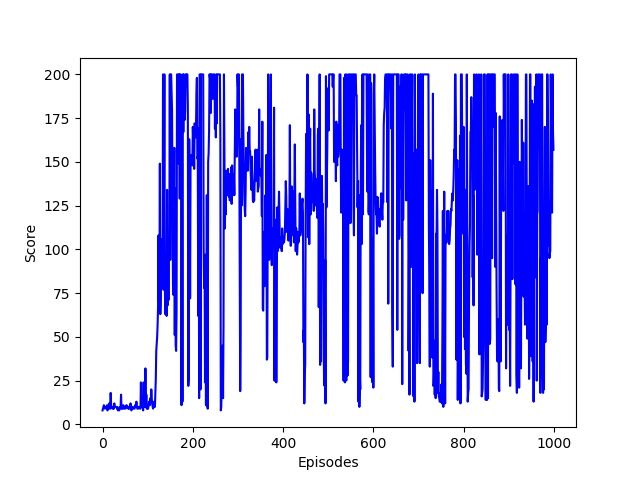
\includegraphics[scale=0.45]{../experiments/discount_factor_095/scores.png}
    \end{minipage}
    \caption{Discount factor: 0.95}
  \end{subfigure}%

  \begin{subfigure}{\textwidth}
    \begin{minipage}{0.5\textwidth}
      \centering
      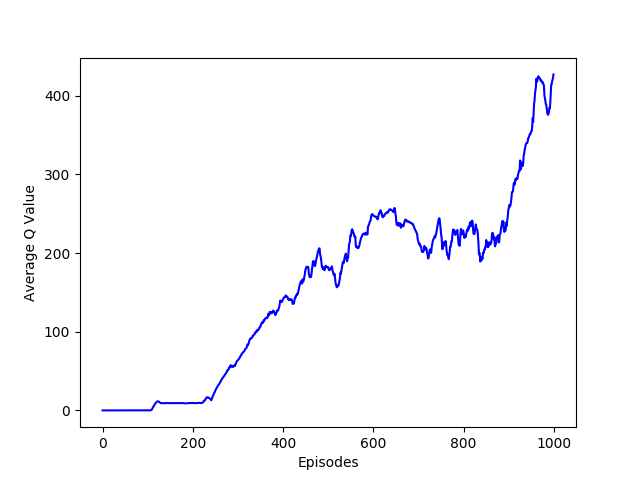
\includegraphics[scale=0.45]{../experiments/discount_factor_0995/qvalues.png}
    \end{minipage}
    \begin{minipage}{0.5\textwidth}
      \centering
      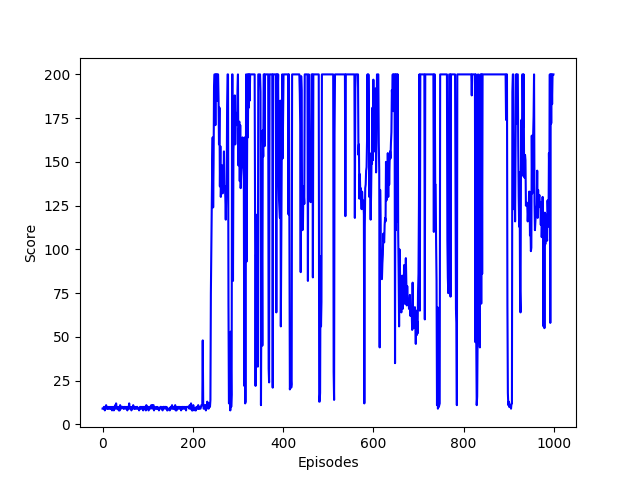
\includegraphics[scale=0.45]{../experiments/discount_factor_0995/scores.png}
    \end{minipage}
    \caption{Discount factor: 0.995}
  \end{subfigure}%

  \caption{Performance under 4 set of discount factors.}
  \label{discount factor}
\end{figure}

From Figure \ref{discount factor}, it is obvious higher discount factor will result in higher average Q
values. The discount factor reflects the importance we put on the future rewards. Thus, by increasing
the discount factor we are able to include more of the future reward which will definitely leads to a
higher total reward than only the current reward. However, when the discount factor is extremely close
to 1, it might not converge as the future reward is almost as important as the current reward. As shown
in Figure \ref{discount factor} (d), the total rewards will keep accumulating with the steps and the Q values
will also keep increasing without converging. As we consider the score as the performance indicator, we
would like to use 0.995 as our discount factor in the final model as it gives more stable performance when it comes to the 
score.

\textbf{Learning rate}

In this section, we have made experiments on 3 set of learning rates: $0.001,0.005,0.01$.
And the results have been drawn in Figure \ref{learning rate}.

\begin{figure}[!htbp]
  \centering
  \begin{subfigure}{\textwidth}
    \begin{minipage}{0.5\textwidth}
      \centering
      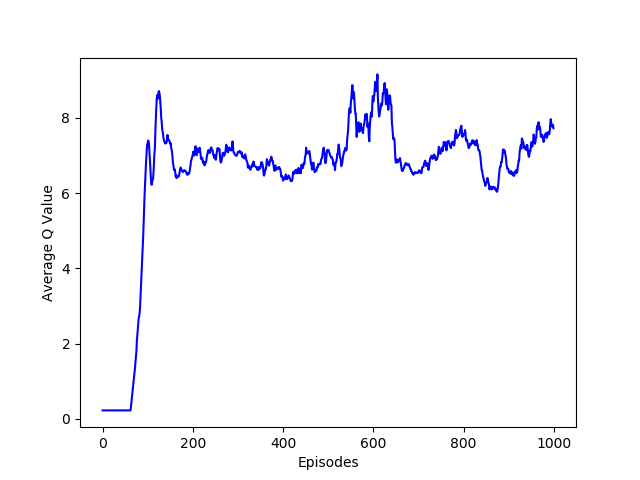
\includegraphics[scale=0.45]{../experiments/lr_1E-3/qvalues.png}
    \end{minipage}
    \begin{minipage}{0.5\textwidth}
      \centering
      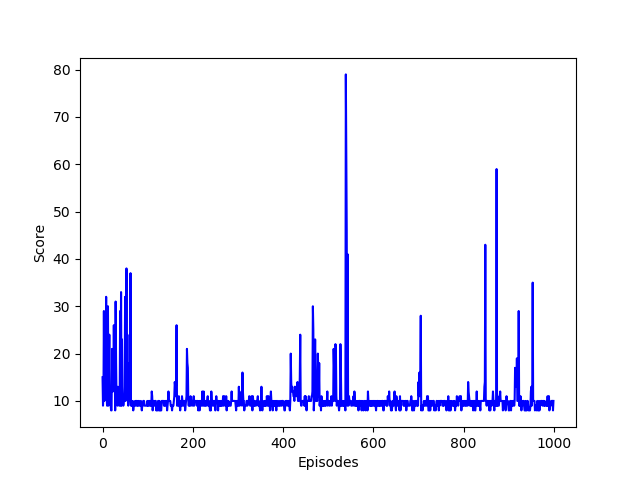
\includegraphics[scale=0.45]{../experiments/lr_1E-3/scores.png}
    \end{minipage}
    \caption{Learning rate: 0.001}
  \end{subfigure}%

  \begin{subfigure}{\textwidth}
    \begin{minipage}{0.5\textwidth}
      \centering
      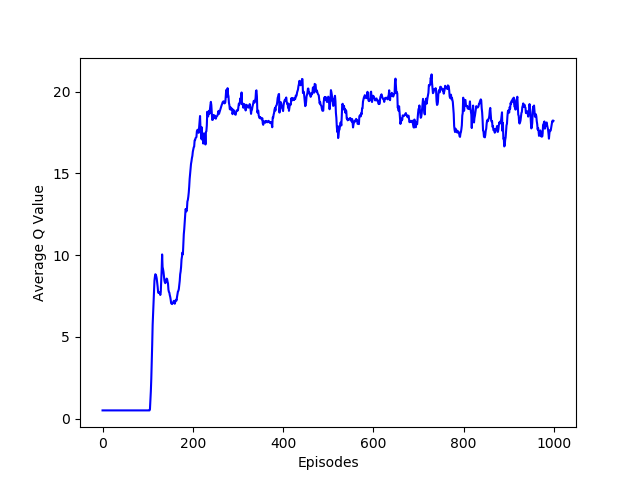
\includegraphics[scale=0.45]{../experiments/lr_5E-3/qvalues.png}
    \end{minipage}
    \begin{minipage}{0.5\textwidth}
      \centering
      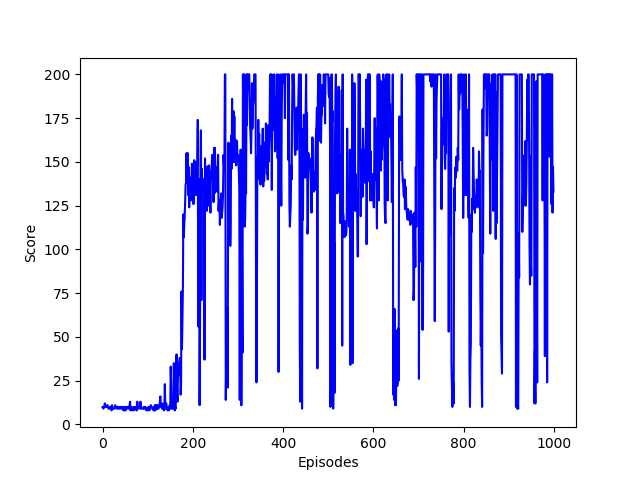
\includegraphics[scale=0.45]{../experiments/lr_5E-3/scores.png}
    \end{minipage}
    \caption{Learning rate: 0.005}
  \end{subfigure}%

  \begin{subfigure}{\textwidth}
    \begin{minipage}{0.5\textwidth}
      \centering
      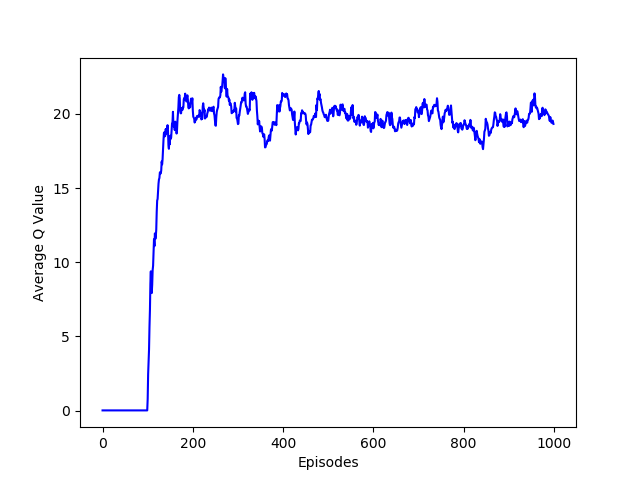
\includegraphics[scale=0.45]{../experiments/lr_1E-2/qvalues.png}
    \end{minipage}
    \begin{minipage}{0.5\textwidth}
      \centering
      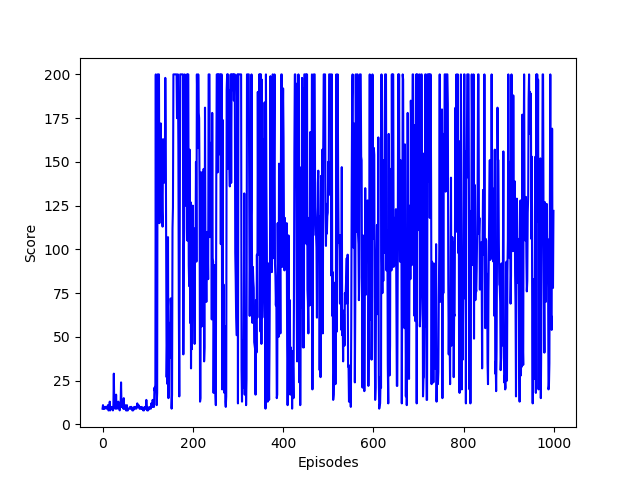
\includegraphics[scale=0.45]{../experiments/lr_1E-2/scores.png}
    \end{minipage}
    \caption{Learning rate: 0.01}
  \end{subfigure}%
  \caption{Performance under 3 set of learning rates.}
  \label{learning rate}
\end{figure}

As we can see in Figure \ref{learning rate}, when the learning rate increases from $0.001$ to $0.005$,
the converged Q value also rises up. And when it increases from $0.005$ to $0.01$,
the converged Q value keeps the same but the episodes for converging are largely decreased.
A higher learning rate will cause a bigger gap between the new and old parameters. Thus with a bigger
learning rate the network will converge much faster. While a low learning rate might cause the model not
converge at all as shown in Figure \ref{learning rate} (a). However, from the scores graphs, it is obvious that
the variance of the scores between episodes has also increased with the learning rate.

\textbf{Memory size}

In this experiment, we have tested 2 memeory sizes: $5000,10000,20000$. The result is shown in Figure
\ref{memory size}.

\begin{figure}[!htbp]
  \centering
  \begin{subfigure}{\textwidth}
    \begin{minipage}{0.5\textwidth}
      \centering
      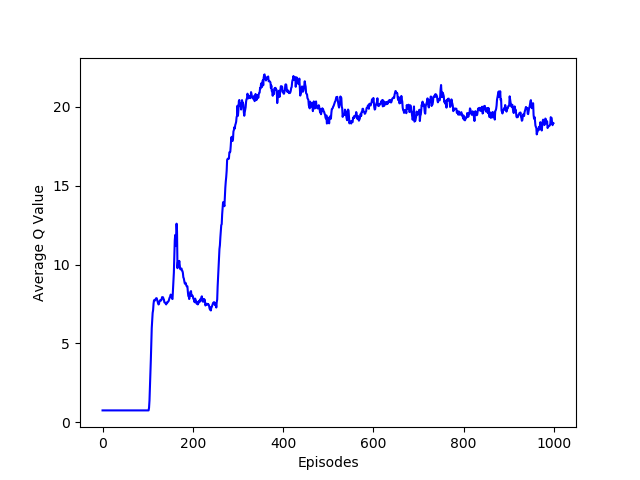
\includegraphics[scale=0.45]{../experiments/mem_size_5000/qvalues.png}
    \end{minipage}
    \begin{minipage}{0.5\textwidth}
      \centering
      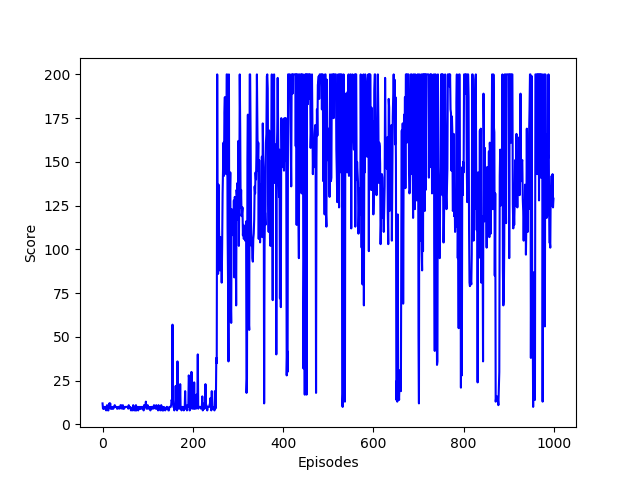
\includegraphics[scale=0.45]{../experiments/mem_size_5000/scores.png}
    \end{minipage}
    \caption{Memory size: 5000}
  \end{subfigure}%

  \begin{subfigure}{\textwidth}
    \begin{minipage}{0.5\textwidth}
      \centering
      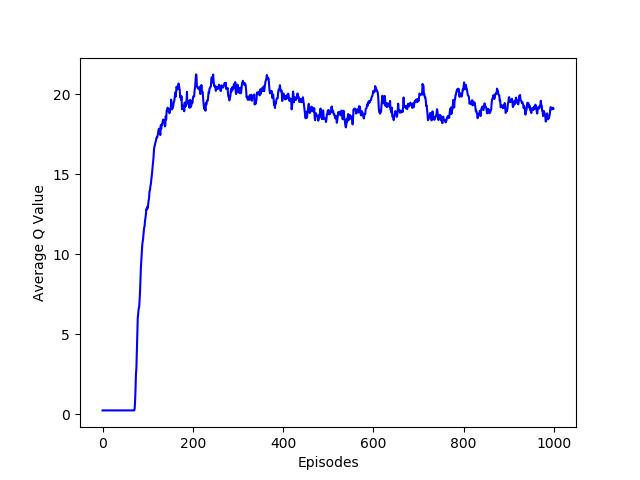
\includegraphics[scale=0.45]{../experiments/mem_size_10000/qvalues.png}
    \end{minipage}
    \begin{minipage}{0.5\textwidth}
      \centering
      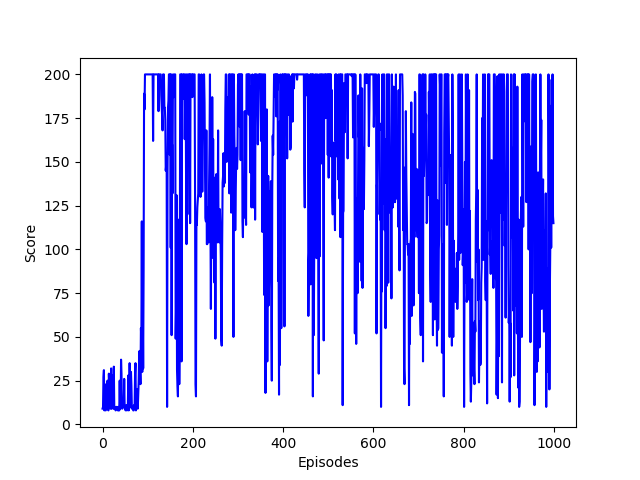
\includegraphics[scale=0.45]{../experiments/mem_size_10000/scores.png}
    \end{minipage}
    \caption{Memory size: 10000}
  \end{subfigure}%

  \begin{subfigure}{\textwidth}
    \begin{minipage}{0.5\textwidth}
      \centering
      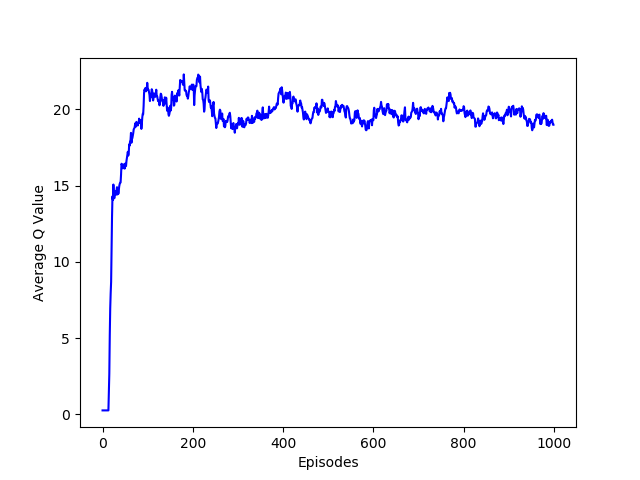
\includegraphics[scale=0.45]{../experiments/mem_size_20000/qvalues.png}
    \end{minipage}
    \begin{minipage}{0.5\textwidth}
      \centering
      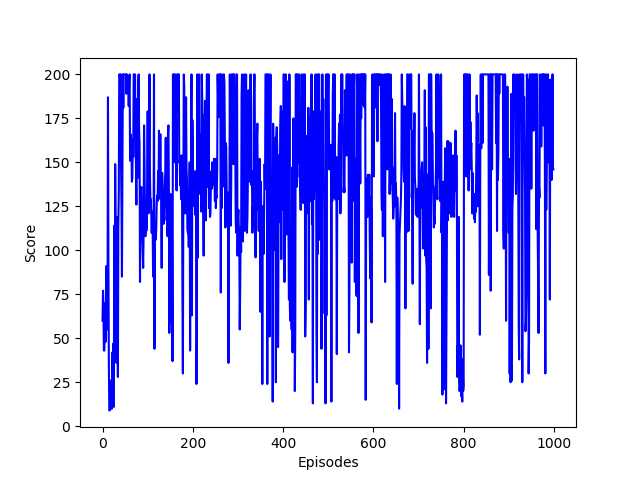
\includegraphics[scale=0.45]{../experiments/mem_size_20000/scores.png}
    \end{minipage}
    \caption{Memory size: 20000}
  \end{subfigure}%
  \caption{Performance under 3 set of memory sizes.}
  \label{memory size}
\end{figure}

It can be seen that the number of episodes for converging decreasing as the memory size increases.
With a bigger memeory size, there will also be more samples used for training each time. Thus it will needed less
episodes for convergence. Besides, the convergence process is also more stable.

\subsection{Impact of the update frequency of target network}

Here we choose 3 set of update frequencies: $1,5,10$, the result of which has been drawn in Figure
\ref{update frequency}.

\begin{figure}[!htbp]
  \centering
  \begin{subfigure}{\textwidth}
    \begin{minipage}{0.5\textwidth}
      \centering
      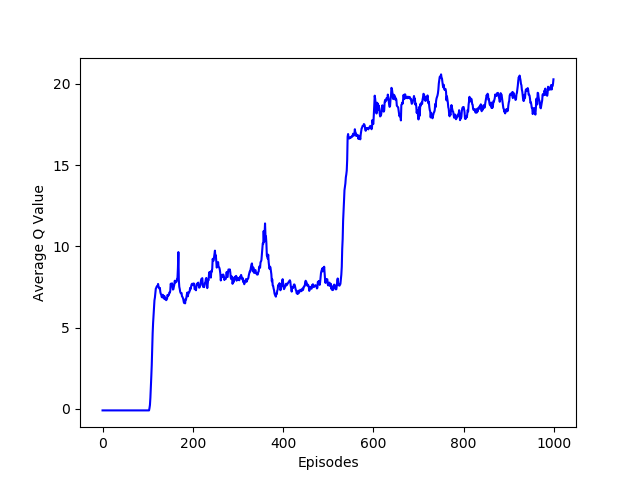
\includegraphics[scale=0.45]{../experiments/update_fq_1/qvalues.png}
    \end{minipage}
    \begin{minipage}{0.5\textwidth}
      \centering
      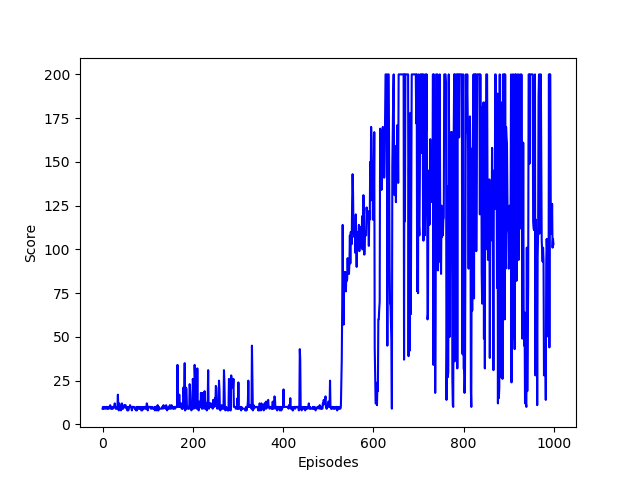
\includegraphics[scale=0.45]{../experiments/update_fq_1/scores.png}
    \end{minipage}
    \caption{Update frequency: 1}
  \end{subfigure}%

  \begin{subfigure}{\textwidth}
    \begin{minipage}{0.5\textwidth}
      \centering
      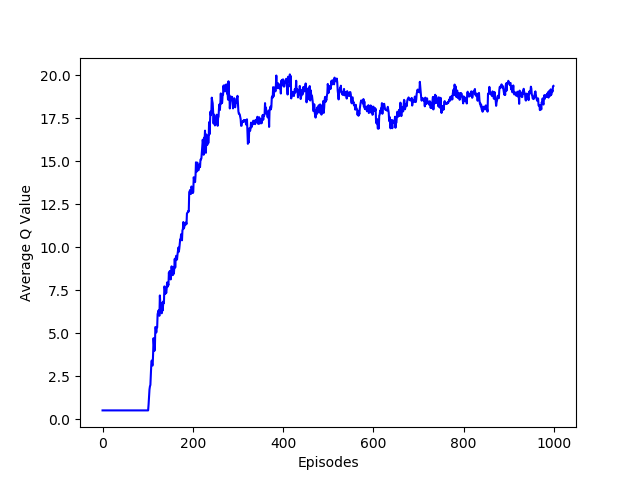
\includegraphics[scale=0.45]{../experiments/update_fq_5/qvalues.png}
    \end{minipage}
    \begin{minipage}{0.5\textwidth}
      \centering
      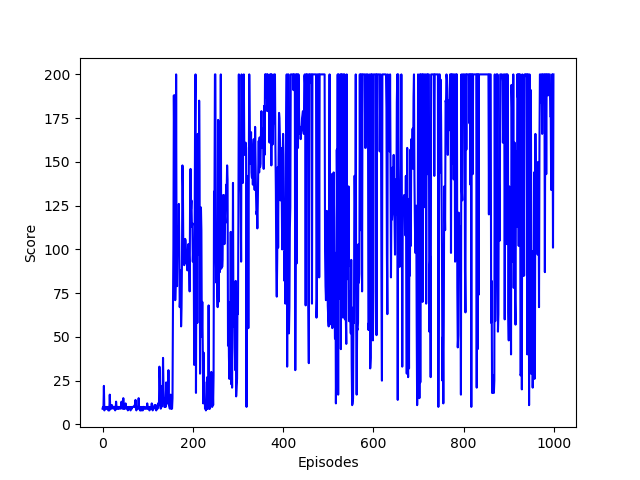
\includegraphics[scale=0.45]{../experiments/update_fq_5/scores.png}
    \end{minipage}
    \caption{Update frequency: 5}
  \end{subfigure}%

  \begin{subfigure}{\textwidth}
    \begin{minipage}{0.5\textwidth}
      \centering
      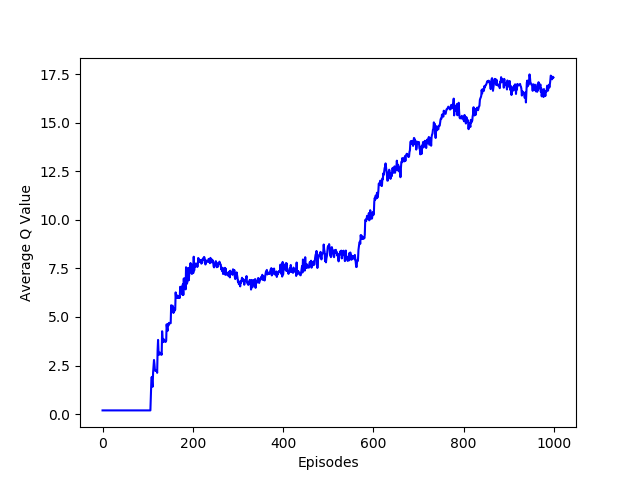
\includegraphics[scale=0.45]{../experiments/update_fq_10/qvalues.png}
    \end{minipage}
    \begin{minipage}{0.5\textwidth}
      \centering
      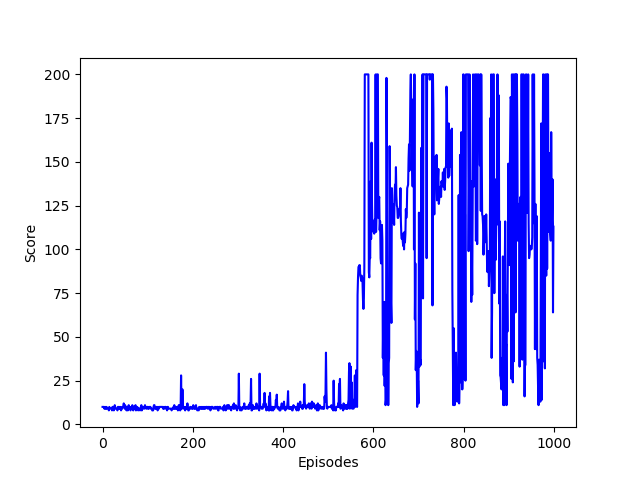
\includegraphics[scale=0.45]{../experiments/update_fq_10/scores.png}
    \end{minipage}
    \caption{Update frequency: 10}
  \end{subfigure}%
  \caption{Performance under 3 set of update frequencies.}
  \label{update frequency}
\end{figure}

The update frequency will control the frequency to update the parameters of the target network.
When it is too high, the network might be stuck in a local optimal point for a long time as shown in
Figure \ref{update frequency} (a). However, when the update frequency is too low as in Figure \ref{update frequency}
(c), it will take much more time to converge.

\subsection{Solve the problem}

According to the above parameter tuning process, we have chosen the optimal parameter setting as in
Table \ref{param table}. And the result is visualized in Figure \ref{final}. In this way, we can get
the maximum average Q values. And after almost 100 episodes, the scores have reached 200.
Finally, the problem solved after 590 episodes.

\begin{table}[H]
  \centering
  \begin{tabular}{cc}
  \hline\hline
  Parameter& Value\\
  \hline\hline
  discount factor & 0.995\\
  learning rate & 0.005\\
  memory size & 20000\\
  target update frequency & 1\\
  \hline
  \end{tabular}
  \caption{Optimal parameter setting}
  \label{param table}
\end{table}

\begin{figure}[H]
  \centering
  \begin{minipage}{0.49\textwidth}
    \centering
    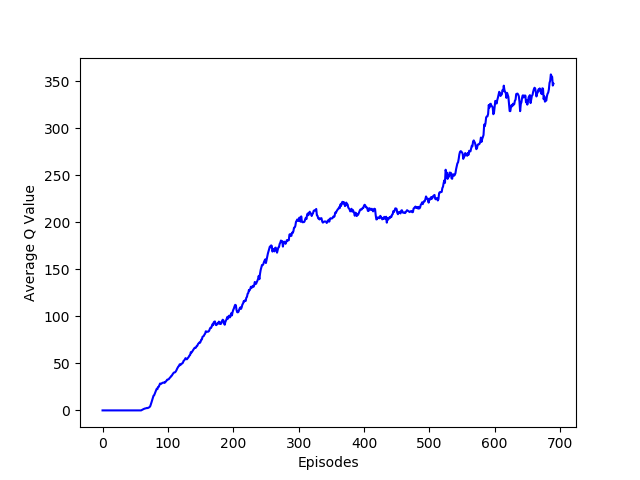
\includegraphics[scale=0.45]{../experiments/final/qvalues.png}
  \end{minipage}
  \begin{minipage}{0.49\textwidth}
    \centering
    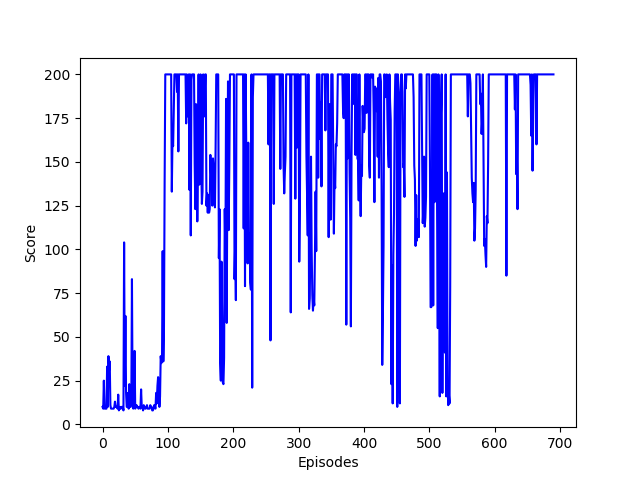
\includegraphics[scale=0.45]{../experiments/final/scores.png}
  \end{minipage}
  \caption{Performance under the optimal parameter setting.}
  \label{final}
\end{figure}

\pagebreak
\appendix
\section{Appendix}
\lstinputlisting{../cartpole_dqn.py}
\lstinputlisting{../utils/csvlogger.py}
\lstinputlisting{../utils/exp_folder.py}
\lstinputlisting{../utils/hparams.py}
\end{document}
